\documentclass[12pt]{article}
\usepackage{amsmath}
\usepackage{graphicx}
\usepackage{hyperref}
\usepackage{listings}
\usepackage{color}
\usepackage{pythonhighlight}

\title{Operating System Course Report - First Half of the Semester}
\author{A class}
\date{\today}

\begin{document}

\maketitle
\newpage

\tableofcontents
\newpage

\section{Introduction}
This report summarizes the topics covered during the first half of the Operating System course. It includes theoretical concepts, practical implementations, and assignments. The course focuses on the fundamentals of operating systems, including system architecture, process management, CPU scheduling, and deadlock handling.

\section{Course Overview}
\subsection{Objectives}
The main objectives of this course are:
\begin{itemize}
    \item To understand the basic components and architecture of a computer system.
    \item To learn process management, scheduling, and inter-process communication.
    \item To explore file systems, input/output management, and virtualization.
    \item To study the prevention and handling of deadlocks in operating systems.
\end{itemize}

\subsection{Course Structure}
The course is divided into two halves. This report focuses on the first half, which covers:
\begin{itemize}
    \item Basic Concepts and Components of Computer Systems
    \item System Performance and Metrics
    \item System Architecture of Computer Systems
    \item Process Description and Control
    \item Scheduling Algorithms
    \item Process Creation and Termination
    \item Introduction to Threads
    \item File Systems
    \item Input and Output Management
    \item Deadlock Introduction and Prevention
    \item User Interface Management
    \item Virtualization in Operating Systems
\end{itemize}

\section{Topics Covered}

\subsection{Basic Concepts and Components of Computer Systems}
This section explains the fundamental components that make up a computer system, including the CPU, memory, storage, and input/output devices.

\subsection{System Performance and Metrics}
This section introduces various system performance metrics used to measure the efficiency of a computer system, including throughput, response time, and utilization.


\subsection{System Architecture of Computer Systems}


Konsep sistem arsitektur komputer merujuk pada desain dan struktur dasar yang menentukan cara kerja komputer, termasuk interaksi antara komponen perangkat keras (hardware) dan perangkat lunak (software). Arsitektur komputer pada dasarnya menjelaskan bagaimana CPU, memori, perangkat input/output, dan komponen lain bekerja sama untuk menjalankan instruksi program. Arsitektur ini mencakup tidak hanya desain fisik bagian-bagian tersebut, tetapi juga bagaimana mereka diatur untuk mencapai kinerja komputasi terbaik.

\subsubsection{Pengertian Sistem Arsitektur Komputer}


Semua komputer, berapa pun ukurannya, didasarkan pada seperangkat aturan yang menyatakan bagaimana perangkat lunak dan perangkat keras bergabung bersama dan berinteraksi untuk membuatnya bekerja. Inilah yang disebut dengan arsitektur komputer. 


Arsitektur komputer juga dapat diartikan sebagai ilmu yang mempelajari tentang cara menghubungkan berbagai komponen perangkat keras, hingga terbentuklah sebuah komputer. Singkatnya, arsitektur komputer terdiri dari beberapa aturan untuk menjalankan dan mengoperasikan sistem.

\subsection{Process Description and Control}
Processes are a central concept in operating systems. This section covers:
\begin{itemize}
    \item Process states and state transitions
    \item Process control block (PCB)
    \item Context switching
\end{itemize}

\subsection{Scheduling Algorithms}
This section covers:
\begin{itemize}
    \item First-Come, First-Served (FCFS)
    \item Shortest Job Next (SJN)
    \item Round Robin (RR)
\end{itemize}
It explains how these algorithms are used to allocate CPU time to processes.

\subsection{Process Creation and Termination}
Details how processes are created and terminated by the operating system, including:
\begin{itemize}
    \item Process spawning
    \item Process termination conditions
\end{itemize}

\subsection{Introduction to Threads}
This section introduces the concept of threads and their relation to processes, covering:
\begin{itemize}
    \item Single-threaded vs. multi-threaded processes
    \item Benefits of multithreading
\end{itemize}

\begin{figure}[h]
    \centering
    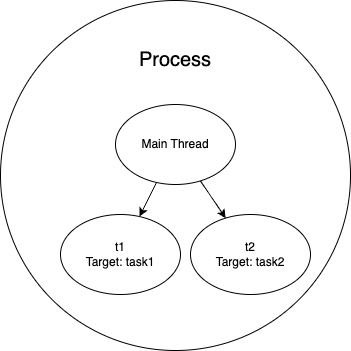
\includegraphics[width=0.5\textwidth]{/Users/khawaritzmi/Unhas/os_report_mid2024/a_class/asset/example.png}  % Sesuaikan nama file dan ukurannya
    \caption{Ini adalah gambar contoh dari multithreading.}
    \label{fig:contoh_gambar}
\end{figure}

Seperti yang terlihat pada Gambar \ref{fig:contoh_gambar}, inilah cara menambahkan gambar dengan keterangan.

\subsection{File Systems}
File systems provide a way for the operating system to store, retrieve, and manage data. This section explains:
\begin{itemize}
    \item File system structure
    \item File access methods
    \item Directory management
\end{itemize}

\subsection{Input and Output Management}
Input and output management is key for handling the interaction between the system and external devices. This section includes:
\begin{itemize}
    \item Device drivers
    \item I/O scheduling
\end{itemize}

\subsection{Deadlock Introduction and Prevention}
Explores the concept of deadlocks and methods for preventing them:
\begin{itemize}
    \item Deadlock conditions
    \item Deadlock prevention techniques
\end{itemize}

\subsection{User Interface Management}
This section discusses the role of the operating system in managing the user interface. Topics covered include:
\begin{itemize}
    \item Graphical User Interface (GUI)
    \item Command-Line Interface (CLI)
    \item Interaction between the user and the operating system
\end{itemize}

\subsection{Virtualization in Operating Systems}
Virtualization allows multiple operating systems to run concurrently on a single physical machine. This section explores:
\begin{itemize}
    \item Concept of virtualization
    \item Hypervisors and their types
    \item Benefits of virtualization in modern computing
\end{itemize}

\section{Assignments and Practical Work}
\subsection{Assignment 1: Process Scheduling}
Students were tasked with implementing various process scheduling algorithms (e.g., FCFS, SJN, and RR) and comparing their performance under different conditions.
\subsubsection{Group 1}
\begin{python}
    class Process:
    def __init__(self, pid, arrival_time, burst_time):
        self.pid = pid
        self.arrival_time = arrival_time
        self.burst_time = burst_time
        self.completion_time = 0
        self.turnaround_time = 0
        self.waiting_time = 0
\end{python}

\begin{table}[htbp] % Optional: For floating position
    \centering
    \begin{tabular}{|c|c|c|} % Defines number of columns and alignment (c = center, l = left, r = right). '|' creates vertical lines.
    \hline
    Header 1 & Header 2 & Header 3 \\ % Column headers
    \hline
    Row 1, Column 1 & Row 1, Column 2 & Row 1, Column 3 \\ % First row of data
    \hline
    Row 2, Column 1 & Row 2, Column 2 & Row 2, Column 3 \\ % Second row of data
    \hline
    \end{tabular}
    \caption{Your table caption} % Optional: For adding a caption
    \label{tab:your_label} % Optional: For cross-referencing the table
\end{table}

\subsubsection{Kelompok 3}
\begin{itemize}
\item Pertanyaan 

Buatlah sebuah kelas Process dalam Python yang memiliki atribut untuk menyimpan pid (Process ID), arrival-time, burst-time, serta atribut tambahan seperti completion-time, turnaround-time, dan waiting-time. Kemudian, buatlah sebuah fungsi untuk menghitung waktu penyelesaian (completion time) dari proses dengan algoritma First Come First Serve (FCFS), dan tampilkan hasilnya.
\end{itemize}
\begin{itemize}
 \item Jawaban
\end{itemize}
\begin{python}
class Process:
    def__init__(self, pid, arrival_time, burst_time):
        self.pid = pid
        self.arrival_time = arrival_time
        self.burst_time = burst_time
        self.completion_time = 0
        self.turnaround_time = 0
        self.waiting_time = 0

    def fcfs_scheduling(processes):
    # Mengurutkan proses berdasarkan arrival_time
    processes.sort(key=lambda x: x.arrival_time)
    
    # Menentukan completion_time, turnaround_time, dan waiting_time
    current_time = 0
    for process in processes:
        if current_time < process.arrival_time:
            current_time = process.arrival_time
        
        process.completion_time = current_time + process.burst_time
        process.turnaround_time = process.completion_time - process.arrival_time
        process.waiting_time = process.turnaround_time - process.burst_time
        
        current_time = process.completion_time

def display_processes(processes):
    print("{:<10} {:<15} {:<15} {:<20} {:<20} {:<20}".format(
        'PID', 'Arrival Time', 'Burst Time', 'Completion Time', 'Turnaround Time', 'Waiting Time'))
    for process in processes:
        print("{:<10} {:<15} {:<15} {:<20} {:<20} {:<20}".format(
            process.pid, process.arrival_time, process.burst_time, process.completion_time, process.turnaround_time, process.waiting_time))

# Contoh proses
processes = [
    Process(1, 0, 4),
    Process(2, 1, 3),
    Process(3, 2, 1),
    Process(4, 3, 2)
]

# Menjalankan algoritma FCFS
fcfs_scheduling(processes)

# Menampilkan hasil
display_processes(processes)
\end{python}
\begin{itemize}
 \item Penjelasan output

 Jawaban dari program di atas adalah bahwa dengan menggunakan algoritma First Come First Serve (FCFS), setiap proses dijadwalkan berdasarkan urutan kedatangan. Setelah proses pertama selesai, proses berikutnya dimulai, dan waktu penyelesaian dihitung berdasarkan burst time (durasi eksekusi) setiap proses. Dalam contoh ini, proses pertama (PID 1) dengan waktu kedatangan 0 dan burst time 4 selesai pada waktu 4, sehingga waktu turnaround-nya juga 4 dan waktu tunggunya 0. Proses kedua (PID 2) yang tiba pada waktu 1 memiliki waktu penyelesaian 7, waktu turnaround 6, dan waktu tunggu 3. Proses ketiga (PID 3) dan keempat (PID 4) dihitung dengan cara yang sama. Output menunjukkan bahwa dengan FCFS, proses-proses dengan waktu kedatangan lebih awal diselesaikan lebih dulu, sementara proses yang datang belakangan harus menunggu proses sebelumnya selesai, menghasilkan waktu tunggu yang lebih tinggi pada proses yang datang belakangan.
\end{itemize}

\subsection{Assignment 2: Deadlock Handling}
In this assignment, students were asked to simulate different deadlock scenarios and explore various prevention methods.
\subsubsection{Kelompok 3}

\begin{itemize}
    \item Pertanyaan
    
    Bagaimana cara membuat dua thread dalam Python yang saling menunggu untuk mengakses dua sumber daya yang berbeda, sehingga menyebabkan deadlock? Jelaskan juga outputnya.
\end{itemize}
\begin{itemize}
    \item Jawaban
\end{itemize}
\begin{python}
    import threading
import time

resource_a = threading.Lock()
resource_b = threading.Lock()

def thread1():
    print("Thread 1: Mengambil Resource A")
    resource_a.acquire()
    time.sleep(1)
    print("Thread 1: Mengambil Resource B")
    resource_b.acquire()  # Deadlock terjadi di sini
    resource_b.release()
    resource_a.release()

def thread2():
    print("Thread 2: Mengambil Resource B")
    resource_b.acquire()
    time.sleep(1) 
    print("Thread 2: Mengambil Resource A")
    resource_a.acquire()  # Deadlock terjadi di sini
    resource_a.release()
    resource_b.release()

t1 = threading.Thread(target=thread1)
t2 = threading.Thread(target=thread2)

t1.start()
t2.start()
t1.join()
t2.join()

print("Program selesai.")
\end{python}
\begin{itemize}
    \item Penjelasan

    Thread 1 berhasil mengunci resource-a dan mencetak pesan bahwa ia telah mengambil Resource A, sementara Thread 2 mengunci resource-b dan mencetak pesan bahwa ia telah mengambil Resource B. Setelah tidur selama 1 detik, Thread 1 mencoba mengunci resource-b, tetapi gagal karena sudah dipegang oleh Thread 2. Demikian pula, Thread 2 mencoba mengunci resource-a, yang sudah dipegang oleh Thread 1. Akibatnya, kedua thread saling menunggu, menyebabkan program terjebak dalam kondisi deadlock, dan tidak mencapai pernyataan "Program selesai." Ini mengilustrasikan bagaimana deadlock dapat terjadi dalam pemrograman multithreading.
\end{itemize}

\subsection{Assignment 3: Multithreading and Amdahl's Law}
This assignment involved designing a multithreading scenario to solve a computationally intensive problem. Students then applied **Amdahl's Law** to calculate the theoretical speedup of the program as the number of threads increased.
\subsubsection{Kelompok 3}

\begin{itemize}
    \item Pertanyaan
    
    Program Python yang menggunakan multithreading untuk menghitung jumlah bilangan genap dan bilangan ganjil dari list yang berisi 1 juta angka. Gunakan dua thread: satu thread untuk menghitung bilangan genap dan satu lagi untuk bilangan ganjil. Terapkan juga hukum Amdhal untuk menghitung kecepatan teoritis.
\end{itemize}
    
\begin{itemize}
    \item Jawaban
\end{itemize}
\begin{python}
import threading
import time

# Fungsi untuk menghitung bilangan genap
def count_even(data, result):
    count = 0
    for num in data:
        if num % 2 == 0:
            count += 1
    result[0] = count

# Fungsi untuk menghitung bilangan ganjil
def count_odd(data, result):
    count = 0
    for num in data:
        if num % 2 != 0:
            count += 1
    result[0] = count

# Fungsi multithreading
def multi_thread(data):
    even_result = [0]
    odd_result = [0]

    t1 = threading.Thread(target=count_even, args=(data, even_result))
    t2 = threading.Thread(target=count_odd, args=(data, odd_result))

    t1.start()
    t2.start()

    t1.join()
    t2.join()

    return even_result[0], odd_result[0]

# Fungsi untuk menghitung speedup Amdahl's Law
def amdahl_speedup(P, N):
    return 1 / ((1 - P) + (P / N))

# List dengan 1 juta angka
data = list(range(1, 1000001))

# Menghitung menggunakan multithreading
start_time = time.time()
even_count, odd_count = multi_thread(data)
multi_thread_time = time.time() - start_time

# Hukum Amdahl dengan 2 thread dan P = 0.95
P = 0.95
N = 2
speedup = amdahl_speedup(P, N)

print(f"Jumlah bilangan genap: {even_count}")
print(f"Jumlah bilangan ganjil: {odd_count}")
print(f"Waktu eksekusi multi-thread: {multi_thread_time:.4f} detik")
print(f"Speedup teoritis menurut Hukum Amdahl: {speedup:.2f}x")
\end{python}
\begin{itemize}
    \item Penjelasan

Program tersebut menggunakan multithreading untuk menghitung jumlah bilangan genap dan ganjil dari list yang berisi 1 juta angka, dengan dua thread yang bekerja secara paralel. Untuk menghitung kecepatan teoritis (speedup) saat menggunakan lebih dari satu thread, diterapkan Hukum Amdahl. Diasumsikan bahwa 95% dari program dapat diparalelkan. Hasil perhitungan menunjukkan bahwa dengan menggunakan dua thread, speedup teoritis sekitar 1.90 kali 
lebih cepat dibandingkan eksekusi pada satu thread. Ini menunjukkan bahwa multithreading dapat meningkatkan kinerja secara signifikan, namun peningkatannya juga dibatasi oleh bagian program yang tidak bisa diparalelkan.
\end{itemize}


\subsection{Assignment 4: Simple Command-Line Interface (CLI) for User Interface Management}
Students were tasked with creating a simple **CLI** for user interface management. The CLI should support basic commands such as file manipulation (creating, listing, and deleting files), process management, and system status reporting.
\subsubsection{Kelompok 3}

\begin{itemize}
    \item Pertanyaan
    
    Bagaimana cara membuat Command-Line Interface (CLI) menggunakan Python untuk manajemen file yang mendukung operasi dasar seperti membuat, menampilkan, dan menghapus file, serta menjelaskan setiap komponen penting dari implementasi tersebut?
\end{itemize}
\begin{itemize}
    \item Jawaban
\end{itemize}
\begin{python}
import argparse
import os

# Fungsi untuk membuat file
def create_file(filename):
    with open(filename, 'w') as file:
        file.write("This is a new file.")
    print(f"File '{filename}' created.")

# Fungsi untuk menampilkan file
def list_files():
    files = os.listdir('.')
    print("Files in the current directory:")
    for file in files:
        print(f"- {file}")

# Fungsi untuk menghapus file
def delete_file(filename):
    try:
        os.remove(filename)
        print(f"File '{filename}' deleted.")
    except FileNotFoundError:
        print(f"File '{filename}' not found.")

# Fungsi utama untuk menjalankan CLI
def main():
    # Menggunakan argparse untuk menangani argumen dari pengguna
    parser = argparse.ArgumentParser(description='Simple CLI for file management.')
    parser.add_argument('command', choices=['create', 'list', 'delete'], help='Command to execute.')
    parser.add_argument('filename', nargs='?', help='Name of the file to manipulate.')

    args = parser.parse_args()

    # Menentukan tindakan berdasarkan argumen yang diberikan
    if args.command == 'create' and args.filename:
        create_file(args.filename)
    elif args.command == 'list':
        list_files()
    elif args.command == 'delete' and args.filename:
        delete_file(args.filename)
    else:
        print("Invalid command or missing filename.")

if __name__ == "__main__":
    main()
\end{python}
\begin{itemize}
    \item Penjelasan

\textit{Command-Line Interface} (CLI) yang dibuat menggunakan Python ini memanfaatkan modul argparse untuk menangani argumen dari pengguna dan modul os untuk melakukan manipulasi berkas. Program ini mendukung tiga operasi dasar: membuat berkas, menampilkan daftar berkas, dan menghapus berkas. Fungsi create-file membuat berkas baru dengan nama yang diberikan, list-files menampilkan semua berkas yang ada di direktori saat ini, dan delete-file menghapus berkas yang ditentukan. Pada fungsi utama (main), program memeriksa perintah yang diberikan oleh pengguna seperti create, list, atau delete, dan menjalankan fungsi yang sesuai. CLI ini memungkinkan pengguna untuk mengelola berkas secara langsung melalui terminal dengan perintah yang sederhana dan praktis.
    
\end{itemize}

\subsection{Assignment 5: File System Access}
In this assignment, students implemented file system access routines, including:
\begin{itemize}
    \item File creation and deletion
    \item Reading from and writing to files
    \item Navigating directories and managing file permissions
\end{itemize}
\subsubsection{Kelompok 3}

\begin{itemize}
    \item  Pertanyaan 
    
    sebuah file bernama report.txt saat ini memiliki izin atau proteksi -rw-r--r-- Berikan penjelasan apa arti bagian dari proteksi tersebut.
\end{itemize}


\begin{itemize}
        \item Jawaban 
        
        - :menandakan bahwa fle tersebut bertipe biasa rw- : pemilik file memiliki hak akses untuk membaca (r) dan mengedit (x), tetapi tidak bisa mealkukan exekusi (x). r-- : grup pengguna hanya memiliki hak akses untuk membaca (r) saja, tanpa bisa mengedit (w), dan mengeksekusi (x). r-- : untuk pengguna lain juga memiliki hak akses hanya untuk membaca (r), tanpa bisa mengeksekusi (x) dan mengedit(r).
    \end{itemize}

\section{Conclusion}
The first half of the course introduced core operating system concepts, including process management, scheduling, multithreading, and file system access. These topics provided a foundation for more advanced topics to be covered in the second half of the course.

\end{document}